\section{Method}
\label{sec:method}

\subsection{Task and evaluation protocol (frozen)}
\label{sec:task}
All experiments use a single frozen task specification---stated in full in
this section and frozen before any model-comparison run---applied to twelve
datasets: the Electricity Transformer Temperature (ETT) family
\citep{zhou2021informer} (ETTh1, ETTh2, ETTm1, ETTm2---7 features each, at
hourly ($h$) and 15-minute ($m$) sampling), the large multivariate sets Electricity (321
channels), Traffic (862), and Weather (21) and the Exchange rates (8,
daily), as benchmarked by \citet{wu2021autoformer} and redistributed by the
Time-Series Library \citep{wu2023timesnet}, Solar-Energy (137, 10-minute)
\citep{lai2018lstnet}, and three mechanistic synthetic families (controlled
sinusoids,
change points, and a delayed-copy task; 7 channels each) generated
deterministically from fixed seeds (Appendix~\ref{sec:appendix-roadmap}).
Each dataset is split chronologically $60\%/20\%/20\%$ into
train/validation/test with stride-1 sliding windows of length $L{=}256$ that
never span a split boundary. Normalization is a per-feature z-score whose
statistics are fit on the \emph{train} split only and applied to all splits
(the earlier practice of fitting over the full series was a future-statistics
leak and is fixed); channels with zero training variance are normalized with
unit scale. The task is \emph{direct} 96-step forecasting: in one forward
pass the model maps an input window $x \in \mathbb{R}^{B \times L \times F}$
to a forecast $\hat{y} \in \mathbb{R}^{B \times H \times F}$, where $B$ is the
number of windows in the batch, $L{=}256$ the lookback, $H{=}96$ the horizon,
and $F$ the number of features (channels) of the dataset. The loss is the
pooled mean squared error (MSE) over all $(B, H, F)$ elements, reported in
standardized units (lower is better).
No autoregressive decoding and no teacher forcing is used. Causality is
enforced by construction and verified empirically: a future-invariance and
exact-zero-future-gradient suite passes for every variant. Windows overlap
by 255/256 positions and are therefore not independent samples; this is a
declared limitation (Section~\ref{sec:limitations}).

Training is identical for every configuration: AdamW ($\mathrm{lr}{=}10^{-4}$,
weight decay $10^{-5}$), gradient clipping at norm 10, batch size 32, a
fixed budget of 10 epochs, float32 on CPU (Apple Silicon, 8 threads), and
deterministic seeding with the same seed used for data loading and model
initialization. The factorial is run at $n{=}25$ paired seeds: the five
pre-registered seeds $\{42, 123, 2024, 7, 99\}$ and a 20-seed power
extension (seeds 1--21 excluding the pre-registered set) run under the
byte-identical protocol and merged post hoc (Section~\ref{sec:rq1}). The
fixed 10-epoch budget is justified by learning-curve
analysis on the pre-registered-seed runs: all cells are in a plateau regime
after epoch 4 and the mean last-3-epoch drift across those 20 runs is
$+0.0009$; no cell keeps improving
systematically, so the budget does not bias cell comparisons.

\subsection{Model family}
\label{sec:family}
All configurations share one minimal Transformer block (hidden size
$d{=}128$, $h{=}4$ heads, head dimension $d_h{=}32$, hence
$d = h\,d_h$) with a horizon head
$\mathrm{Linear}(128 \rightarrow H \cdot F)$ applied to the last position:
\begin{equation}
e = \mathrm{input\_proj}(x) + \mathrm{pos\_embedding}, \qquad
z = \mathrm{MLP}(\mathrm{LN}(\mathrm{attn}(e) + e)), \qquad
\hat{y} = \mathrm{horizon\_head}(z[:, -1, :]),
\end{equation}
where $x$ is the input window of Section~\ref{sec:task}, $e$ the embedded
sequence, $\mathrm{LN}$ layer normalization, $\mathrm{MLP}$ the
feed-forward block, and $z$ the block output; $z[:, -1, :]$ is its last
position, the only position the forecast head reads. The only difference
between configurations is the attention module. The shared Q/KV/O
(query, key--value, output) projections follow the MLA-style pattern: a
low-rank query projection with root-mean-square normalization (RMSNorm), a
tied single-head KV projection ($K = V$) with rotary position embeddings
(RoPE) applied to the last 8 of the $d_h{=}32$ dimensions, and a grouped
output projection.
A full causal attention variant (\emph{Normal}) with no compression serves
as the task-appropriate baseline.

Figure~\ref{fig:arch} draws the two paths side by side at the same level of
detail, so that the quantity that separates the two families---how many key
columns a query reads---can be read from the figure rather than inferred from
the prose. Panel~(a) reads all $L$
columns under a causal mask. Panel~(b) reads a column set assembled from
three sources---$L/c_{KV}$ compressed blocks, the last $W{=}16$ positions
kept at full resolution, and one learned sink---and each attention box
carries a strip marking those columns. Two properties of panel~(b) carry
into the rest of the paper. Its per-query column count grows as $L/c_{KV}$
plus a constant (the window and the sink), rather than as $L$, so at fixed
rates the saving is a constant factor and not a change of asymptotic order;
Section~\ref{sec:forecast} therefore reports it as a ratio that saturates
rather than as a speedup that compounds with context. And the selection is
applied as a mask rather than as a reduction in work---every block column is
computed either way---so the arithmetic is set by the two rates and not by
which blocks are kept, and what the selection does buy is measured in
Section~\ref{sec:controls}.

\begin{figure}[t]
\centering
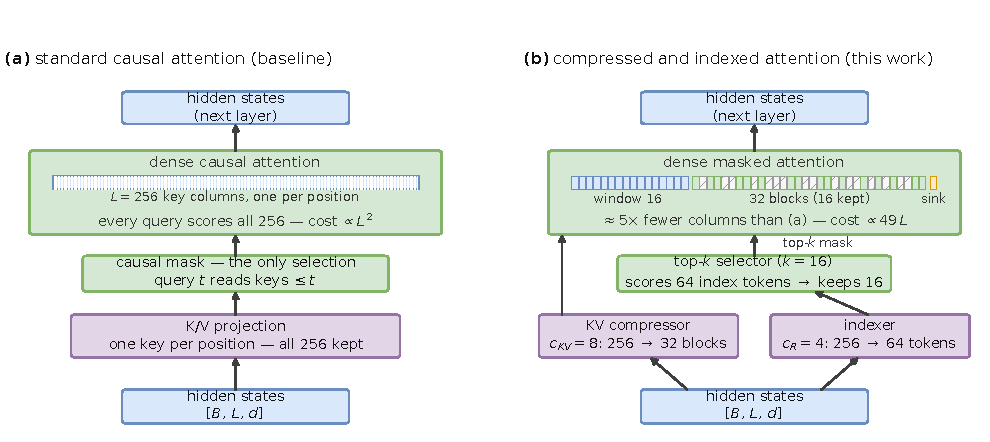
\includegraphics[width=\linewidth]{figures/fig1_architecture_compare.pdf}
\caption{The attention module, standard beside compressed. Both panels start
from the same hidden-state tensor $[B, L, d]$ ($B$ = batch size, $L$ =
lookback, $d$ = hidden size) and feed the next layer. \textbf{(a)}~Standard
causal attention, the \emph{Normal} baseline: every position keeps its own key
and value, so each query scores all $L{=}256$ keys, restricted only by the
causal mask---cost growing with $L^2$. \textbf{(b)}~The compressed-and-indexed
module, drawn at the $(c_{KV}, c_R) = (8,4)$ cell ($c_{KV}$ = KV-cache
compression rate, positions per stored block; $c_R$ = routing resolution,
positions per index token). From the same hidden states, two branches run in
parallel: a KV compressor ($c_{KV}{=}8$: 256 positions $\to$ 32 blocks) and a
routing indexer ($c_R{=}4$: 256 positions $\to$ 64 index tokens). The router
scores the index tokens with the query and keeps the top-$k{=}16$; two index
tokens map to one block at this cell, so up to 16 of the 32 block columns are
attended. The 32 block columns, the sliding window (16 uncompressed
positions) and an always-visible sink column are combined into a fixed column
set of $16 + 32 + 1 = 49$, and attention is computed densely over that set
with unselected blocks masked to $-\infty$ (Section~\ref{sec:family-mech});
the hatched cells are the ones computed and then masked. Cost therefore
scales with the strip's width, 49 against 256, not with the selection. Both panels
share the Transformer block and the Q/KV/O projections; only the attention
module differs, and the horizon head maps the last hidden state to the
96-step forecast.}
\label{fig:arch}
\end{figure}

\subsection{The compressed-and-indexed attention family}
\label{sec:family-mech}
Each compressed configuration (Figure~\ref{fig:arch}) consists of three
components, all inherited verbatim from the reference implementation:

\textbf{Two-series compressor.} The $L$ positions are projected to double
width and gated by a per-dimension softmax over $2m$ slots, so that every
token contributes to two adjacent windows (its own and the next); the
weighted sum is RMSNormed and RoPE-encoded at block starts. With rate
$m$---the cell's KV compression rate, $m = c_{KV}$---this yields
$C = L/m$ KV blocks, block $j$ covering $[mj, mj + m - 1]$. The
same compressor, with its own parameters, produces the $M = L / m_{idx}$
routing index tokens, where $m_{idx} = c_R$ is the routing resolution. The
two rates are the only quantities the factorial varies
(Section~\ref{sec:factorial}); $C$ and $M$ are the column counts they imply.

\textbf{Router (scorer + top-$k$ selector).} Each query vector $q$ (one per
head, of dimension $d_h$) scores all $M$ index tokens as
$\mathrm{ReLU}(q \cdot \mathrm{idx}^\top)/\sqrt{d_h}$, where
$\mathrm{idx}$ denotes the index-token matrix and
$\mathrm{ReLU}(z) = \max(z, 0)$; the per-head scores are combined by a
head-mixing weight that is fixed in practice (see the trainability note
below). The router masks tokens that lie in the future and selects the
top-$k$ ($k{=}16$) of the remaining ones. We use ``router'' for the scorer-plus-selector
combination; DeepSeek-V4 \citep{deepseekv4_2026} calls the analogous scorer
the \emph{Lightning Indexer} and the selection step the \emph{top-$k$
selector} (their paper uses neither ``router'' nor a standalone indexer
module feeding the selector --- the indexer scores the KV entries, which the
selector then subsamples). In all compressed configurations the router reuses the
main query (shared-Q), valid because the query head dimension equals the
index head dimension; this removes one projection and one RoPE application.
The hard top-$k$ selection is non-differentiable, so the indexer parameters
(including CSA's dedicated $\mathrm{idx\_q\_proj}$) receive zero task-loss
gradient: no learning signal reaches the selector, and ``routing granularity'' effects in
this paper are selection-architecture effects, not learned routing. The released audit
logs both a zero gradient norm and a zero optimizer update delta for every
indexer-exclusive parameter, so those parameters are tracked by the optimizer rather
than absent from the graph. The audit
establishes gradient isolation, not literal route constancy---index scores are
computed from features produced by trainable upstream components, so the selected
set can change as those features drift over training. A route-overlap probe across
epochs measures that drift rather than assuming it away (Section~\ref{sec:probes});
a trained selector remains deferred future work (both audit limits are in the
released logs).

\textbf{Dense masked attention over the sparse selection.} Instead of
gathering the selected blocks, attention is computed densely over a fixed
column set---the $C$ KV blocks plus a sliding window of $W{=}16$---with
$-\infty$ masking of unselected blocks and a single learnable ``sink''
softmax column for stability. Masking to $-\infty$ makes the dense result
exactly equal to the sparse top-$k$ selection, with no approximation. On
CPU this formulation is several times faster than per-query gather in our
implementation, and it keeps the softmax exact.

\textbf{Index-to-block mapping (per cell).} The router selects top-$k{=}16$ index
tokens; index token $t$ covers $[4t, 4t{+}3]$ at $c_R{=}4$ ($[8t, 8t{+}7]$ at $c_R{=}8$)
and must be translated to KV-block id $j$ before the dense masked attention
($\sslash$ below denotes integer division):
\begin{itemize}
  \item $(8,4)$: two fine tokens per coarse block --- block $j = t \sslash 2$,
        covering $[8j, 8j{+}7]$ (at most two of the 16 selections collide per block).
  \item Equal-rate cells $(4,4)$, $(8,8)$: token $t$ \emph{is} block $t$ (identity).
  \item $(4,8)$: one coarse token fans out to two fine blocks $(2t, 2t{+}1)$,
        doubling the per-query selection to 32 block slots.
  \item Deeper ratios ($(16,4)$, $(32,4)$): $p$ fine tokens per coarse block --- block
        $j = t \sslash p$ with $p = 4, 8$ (the general many-to-one rule).
\end{itemize}
A selected block is read only when its entire span ends at or before the query
($\mathrm{block\_end} \le$ the query's position); otherwise --- and for tokens masked as future or
out of range --- it maps to a sentinel id that \_attend drops, so no query reads
future positions. Causality holds through the overlapping compressor as well: each
compressed block mixes only its own and the previous window (receptive field
$[m(j{-}1), mj{+}m{-}1]$), i.e.\ strictly backward, so the block-end guard is
sufficient. Any other $(c_{KV}, c_R)$ geometry raises instead of guessing a mapping
(the general rule above covers every tested cell).
The per-cell rule is exercised by a regression test at every tested rate pair and
at non-divisible token counts (Appendix~\ref{sec:appendix-repro}); an earlier
implementation applied the $(8,4)$ rule to every geometry, which is why the three
affected cells reported in Section~\ref{sec:experiments} are re-runs.

\subsection{The two design axes and the factorial}
\label{sec:factorial}
The two axes are the KV compression rate $c_{KV} = m$ and the routing
resolution $c_R = m_{idx}$. We evaluate the $2 \times 2$ factorial over
$c_{KV}, c_R \in \{4{:}1, 8{:}1\}$, i.e.\ cells $(4,4)$, $(8,4)$, $(4,8)$,
$(8,8)$. The two corners that also appear in the cross-dataset study are
referred to by name throughout:
\begin{itemize}
  \item \textbf{CSA} --- the equal-rate corner $(4,4)$, in which both axes
        sit at $4{:}1$. We adopt the \emph{name} of DeepSeek-V4's Compressed
        Sparse Attention \citep{deepseekv4_2026}, whose rate design point
        this cell matches: KV compression at rate $m{=}4$ (the same value used
        in DeepSeek-V4-Flash/Pro), routing/selection over entries at the
        same $4{:}1$ granularity, and a local sliding-window branch. The
        name marks the configuration, not an equivalence claim: we evaluate
        our own implementation at $L{=}256$ scale (selection budget
        $k{=}16$, window 16, versus their $k{\in}\{512, 1024\}$, window
        128), not DeepSeek-V4's mechanism (Section~\ref{sec:related}).
  \item \textbf{DRRA (Dual-Rate Routed Attention)} --- the dual-rate corner
        $(8,4)$ (coarse content, fine routing), which gives the family its
        working name. We use ``champion'' for this cell strictly as shorthand for
        ``the dual-rate corner'' (its efficiency geometry, not accuracy rank: on validation
        no cell is best, DRRA-vs.-CSA exact Wilcoxon $p = 0.62$); everywhere else we name
        the cell explicitly.
\end{itemize}
The remaining corners $(4,8)$ and $(8,8)$ appear only in the factorial.

\textbf{Why only $\{4,8\}^2$?} The grid is the pre-registered design (frozen
before any run), and a $2\times2$ factorial is the minimal design that
identifies both main effects and their interaction --- exactly the three
fixed effects of the deferred mixed-effects model. Grid extension was a
deliberate exclusion, for three reasons. First, the natural next points are
degenerate rather than informative: at $c_R{=}16$ the indexer stream has
only $L/16 = 16$ tokens, so the top-$k{=}16$ router selects \emph{all} of
them and routing collapses to attend-to-everything --- a $(\cdot,16)$ cell
would measure the no-routing endpoint, not finer routing (measuring the
latter would require raising $k$ as well, breaking the auxiliary-identical
contract that pairs all cells). Symmetrically, at $c_{KV}{=}16$ the KV
blocks ($16$) no longer outnumber the sliding window ($16$), so the column
composition changes what is being measured. Second, the two levels bracket
a $2\times$ range around the operating region of interest (the CSA corner
$(4,4)$ matches DeepSeek-V4's $m{=}4$), and both effect signs are
established within the bracket. Behavior outside the bracket was extrapolation
at pre-registration time; two deeper ratios, $(16,4)$ and $(32,4)$, were run later as
exploratory probes (same protocol) and are reported separately from the confirmatory
factorial (Section~\ref{sec:rq1}, Appendix~\ref{sec:appendix-exploratory}). The grid remains valid as the confirmatory design: the probes stay exploratory and never enter the confirmatory contrasts. Third, budget: each additional cell costs 25
paired runs ($\approx 6$ h CPU at the measured per-run cost of the seed
extension), and the $2\times2$ spends that budget on replication ---
statistical power for the pre-registered contrasts --- rather than on extra
cells. Adding off-grid cells (e.g.\ the $(\cdot,16)$ endpoint ablation,
roughly 1--2 h for 5 paired seeds) is straightforward in the harness and is
itemized as future work.
Table~\ref{tab:configs} lists the resulting geometry and
parameter counts.

\begin{table}[t]
\centering
\small
\caption{Configuration geometry and parameters (measured; attention module
and full model). All compressed cells share the auxiliary contract
(window 16 = tokens visible to every query, top-$k$ 16 = best-scoring index
tokens routed per query, 4 heads, head dimension 32, hidden 128, shared-Q
= one query projection shared by router and attention,
query/output projection ranks 64 = low-rank bottleneck dimensions) and differ only in
$(c_{KV}, c_R)$ = (KV-cache compression rate, routing resolution, in
positions per stored block and per index token); the low-rank
bottlenecks are equalized to within $0.27\%$ of the $(8,4)$ reference;
results for all cells are in Table~\ref{tab:factorial}. Starred rows are post-hoc exploratory probes, excluded from
all confirmatory contrasts. Columns: $C$ = KV blocks, $M$ = index tokens,
\emph{softmax cols} $= C + W + 1$ = KV blocks $+$ 16-token window $+$
always-visible sink column. Normal
attends to all 256 columns with no sink.}
\label{tab:configs}
\begin{tabular}{lcccccc}
\toprule
Config & $c_{KV}$ & $c_R$ & KV blocks $C$ & Index tokens $M$ & Softmax cols & Params (attn / full) \\
\midrule
Normal & --- & --- & --- & --- & 256 & 102{,}496 / 355{,}200 \\
$(4,4)$ & 4 & 4 & 64 & 64 & 80 + 1 & 95{,}396 / 348{,}100 \\
$(8,4)$ & 8 & 4 & 32 & 64 & 48 + 1 & 95{,}652 / 348{,}356 \\
$(4,8)$ & 4 & 8 & 64 & 32 & 80 + 1 & 95{,}652 / 348{,}356 \\
$(8,8)$ & 8 & 8 & 32 & 32 & 48 + 1 & 95{,}908 / 348{,}612 \\
$(16,4)^*$ & 16 & 4 & 16 & 64 & 32 + 1 & 96{,}164 / 348{,}868 \\
$(32,4)^*$ & 32 & 4 & 8 & 64 & 24 + 1 & 97{,}188 / 349{,}892 \\
\bottomrule
\end{tabular}
\end{table}

\textbf{Reading the table.} Normal is the uncompressed reference: it
attends to all 256 columns and carries 102{,}496 attention parameters.
Every compressed cell shares the identical auxiliary contract (window 16,
top-$k$ 16, 4 heads, hidden 128, shared-Q, ranks 64) and differs only in
the two rates. $c_{KV}{=}8$ halves the number of KV blocks (32 vs.\ 64) and
thereby the softmax columns ($48{+}1$ vs.\ $80{+}1$; 256/49 complete columns,
i.e.\ 5.22$\times$
fewer than Normal); $c_R$ sets how many routing candidates the router
selects from (64 for $c_R{=}4$, 32 for $c_R{=}8$) without changing the
attention cost. The four factorial cells carry $6.4$--$6.9\%$ fewer attention
parameters than Normal (the low-rank $q$/$o$ bottlenecks replace dense
projections), and the exploratory cells $5.2$--$6.2\%$ fewer; full-model counts
are ${\sim}2\%$ below Normal's. The DRRA $(8,4)$ cell therefore combines the smallest attention geometry among the
factorial cells with the fine-router candidate count. Realized routing is sparser than the dense-masked budget (about 14 of 64 unique blocks for equal-rate cells, about 10 of 32 for the dual-rate cell; compute still pays the dense-masked width).

\textbf{Parameter equalization.} The factorial is pre-registered with an
auxiliary-identical contract: all cells share window, top-$k$, heads, hidden
size, optimizer, and schedule, and differ only in $(c_{KV}, c_R)$--the cell
definition. Because the position-bias terms of the two compressors grow with
their rates, attention-parameter counts differ slightly between cells; the
only free compute-quality knobs not part of the cell definition (the
low-rank $q$ and $o$ bottlenecks) are fixed at the DRRA $(8,4)$ ranks
$(64, 64)$, which is the lattice minimum for \emph{every} factorial cell. Each
factorial cell's attention-parameter count deviates from the $(8,4)$ reference
by at most $0.268\%$ (full-model $0.073\%$), well inside the pre-registered
$0.5\%$ tolerance; the exploratory cells keep the same ranks with disclosed
deviations ($+0.54\%$, $+1.6\%$).

\textbf{Complexity.} Attention cost per query is proportional to the number
of softmax columns: 256 for Normal, 80 for $c_{KV}{=}4$ cells, 48 for
$c_{KV}{=}8$ cells (5.22$\times$ fewer complete columns than Normal), and 32/16 for the
exploratory $(16,4)$/$(32,4)$ cells, giving
$O(L \, C_{\mathrm{cols}} \, d)$ per sequence for the score/value
computation, where $C_{\mathrm{cols}} = C + W + 1$ is the softmax-column
count listed in Table~\ref{tab:configs}. The router, however, compares every query against
$M = L/c_R$ index tokens, $O(L \cdot M) = O(L^2/c_R)$: the total
attention-path cost is therefore \emph{quadratic in $L$ with a reduced
constant} ($1/c_R$ on the routing term), \emph{not} subquadratic. Routing
cost is identical for the two $c_R{=}4$ cells regardless of $c_{KV}$. These
are structural facts; measured mean latency, batch scaling, and empirical
log-log slopes are reported in Section~\ref{sec:efficiency}
(Tables~\ref{tab:speed}, Figure~\ref{fig:latency-scale}); FLOPs and memory
accounting are reported there as well. Cross-hardware transfer and
depth/width ablations are conscious scope exclusions of this study
(single machine; single-block architecture), left to future work.
